% !TeX spellcheck = en_GB
\documentclass[12pt,a4paper,twoside]{article}
\usepackage[english]{babel}
\usepackage{amsmath}
\usepackage{amsthm}
\usepackage{amssymb}
\usepackage{amsfonts}
\usepackage{graphicx}
\usepackage{mathtools}
\usepackage[utf8]{inputenc}
\usepackage{csquotes}
\usepackage[hidelinks, final]{hyperref}
\usepackage[printonlyused]{acronym}
\usepackage{color}
\usepackage{transparent}
\graphicspath{{img/}}
\usepackage[%
backend=biber,
url=false,
style=numeric,
sorting=none,
maxnames=4,
minnames=3,
maxbibnames=99,
giveninits,
uniquename=init]{biblatex}
\addbibresource{bachelor_thesis_julien_caselmann.bib}
%TODO: many weird sources, fix them

\newtheorem{definition}{Definition}[section]
\newtheorem{thm}{Theorem}[section]
\newtheorem{lem}{Lemma}[section]
\newtheorem{prop}{Proposition}[section]
\newtheorem{claim}{Claim}[section]
\newtheorem{model}{Model}[section]

\setlength{\voffset}{-28.4mm}
\setlength{\hoffset}{-1in}
\setlength{\topmargin}{20mm}
\setlength{\oddsidemargin}{25mm}
\setlength{\evensidemargin}{25mm}
\setlength{\textwidth}{160mm}

\setlength{\parindent}{0pt}

\setlength{\textheight}{235mm}
\setlength{\footskip}{20mm}
\setlength{\headsep}{50pt}
\setlength{\headheight}{0pt}


\begin{document}
\pagestyle{empty}
%%%% Title page
\begin{titlepage}
\begin{center}

\includegraphics{img/TUMlblack.png}\\[3mm]
\sf
{\Large
  Technische Universit\"at M\"unchen\\[5mm]
  Department of Mathematics\\[8mm]
}
\normalsize
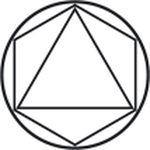
\includegraphics{img/TUMlMblack.png}\\[15mm]

Bachelor's Thesis\\[15mm]

{\Huge
  The Dynamics of Vaccination Hesitancy
}
\bigskip

\normalsize

Julien Caselmann
\end{center}
\vspace*{75mm}

Supervisor: Prof. Dr. Johannes M\"uller
\medskip

Advisor: Prof. Dr. Johannes M\"uller
\medskip

Submission Date: 01.07.2020

\end{titlepage}
%%%% The following has to be signed by hand!

\vspace*{150mm}

I assure the single handed composition of this bachelor's thesis only supported by declared resources.
\bigskip

Munich,
\newpage
%%%% Summary in german
\section*{Zusammenfassung}
Bei einer in englischer Sprache verfassten Arbeit muss eine Zusammenfassung in deutscher Sprache vorangestellt werden.
Daf\"ur ist hier Platz.

\newpage
\tableofcontents
\newpage

%%%% Page numbering restarts here
\pagenumbering{arabic}
\pagestyle{headings}

\newpage

%if you do not use this, delete following packages in preamble:
%acronym

\section*{Abbreviations}
\begin{acronym}[KPMG]%write longest acronym here for nice formatting purposes
	%to use them write \ac{KPMG} or \acp{KPMG for plural in the text}
	\acro{KPMG}{KPMGeneral}
	\acro{SIR}{Susceptibles, Infecteds, Recovereds}
	\acro{BCM}{bounded-confidence model}
	\acro{WHO}{World Health Organization}
	\acro{BVM}{biased voter model}
	%if one acronym's plural form is more than just an "s" attached, you have to specify that:
	\acro{SQ}{sexy query}
	\acroplural{SQ}[SQs]{sexy queries}
\end{acronym}

\section{Introduction}
Impfgegner: (nur 3-5\% in dütschland \cite{Meyer2004}).\\
Sind sehr gefährlich wegen emotive appeals und allg. rhetorical appeals, zitieren medizinische studien und ziehen dann falsche schlüsse (was den meisten nicht auffällt, da paper für den laien schwere kost sind) \cite{Davies2002}.\\
Krankheiten die durch impfung ausgerottet werden können, brechen in religiösen kreisen aus \cite{Novotny1988}.\\
%How to input a inkscape image:
%\begin{figure}
%	\centering %(or not)
%	\def\svgwidth{175pt}
%	\input{foo/bar/file.pdf_tex}
%	\caption{example}
%	\label{fig:example}
%\end{figure}

\section{Mathematical Tools}
%TODO: prolly nur sachen aus my model bifurcation analysis, davor sehe ich NOCH keine verwendung von mathe lul
\section{Hesitancy Model}
Firstly, we will have to take a look at a way to model vaccination hesitancy and try to understand, how the ``vaccinators" behave and where the dependencies of their behaviour lie. The medical/biological approach over the past few years has inter alia been to compose literature reviews and to form working groups such as in \cite{MacDonald2015} to be able to define so-called ``vaccine hesitancy determinants". Those are categories of reasons, for which individuals would decide not to take a vaccine. Then, a mathematical model of the dynamics had to be found, which takes into account the found determinants and one can analyse mathematically to potentially define explicit influence factors for the vaccine hesitancy dynamics. 

Over time, several different models have been elaborated, but only one will be presented in this thesis: the significant work of Bauch and Bhattacharyya in \cite{Bauch2012}. They developed a behaviour-incidence model with the aim to describe the dynamics of the number of vaccinators $x$ depending on different factors such as vaccine risk, efficacy and the number of infectious persons. To get a better overview, all of the variables used in the model will be listed here:
\begin{align}\label{table:bauch_model_variables}
\begin{split}
S &: \textnormal{number of susceptible individuals in the population}\\
I &: \textnormal{number of infected individuals in the population}\\
x &: \textnormal{relative number of vaccinators in the population}\\
\mu &: \textnormal{birth and death rate of the population}\\
\epsilon &: \textnormal{vaccine efficacy}\\
\beta &: \textnormal{infection rate}\\
\tau &: \textnormal{case importation rate}\\
\gamma &: \textnormal{recovery rate}\\
\kappa &: \textnormal{scale factor}\\
\omega &: \textnormal{vaccine penalty}
\end{split}
\end{align}

The vaccine penalty $\omega$ basically describes the amount of risk a vaccination brings and $\kappa$ is a measure for the response speed of the population to external influences. A high value for $\kappa$ means that they change their opinion (pro-vaccine $\rightleftarrows$ contra-vaccine) immediately, a low $\kappa$ stands for a very slow reaction. The variables $S$ and $I$ follow the convention from the well-studied \ac{SIR} model developed by Kermack and McKendrick in 1927 (for more details, see \cite{Muller2015}). We may now define the model:
\begin{model}[\textbf{Behaviour-incidence model by \cite{Bauch2012}}]\label{model:bauch}
	Let the context be defined as in \eqref{table:bauch_model_variables}. Then, the dynamics of the according behaviour-incidence model are:
	\begin{align}
	\begin{split}
	\frac{dS}{dt} &= \mu\left(1-\epsilon x\right) - \mu S - \beta SI - \tau S\\
	&\\
	\frac{dI}{dt} &= -\mu I + \beta SI - \gamma I + \tau S\\
	&\\
	\frac{dx}{dt} &= \kappa x\left(1 - x\right)\left(I - \omega\right)
	\end{split}
	\end{align}
\end{model}

The modelling idea is that every person starts in the group of susceptibles $S$ and either stays in $S$, moves to the group of infecteds $I$, or gets the vaccine and immediately jumps into the group of recovereds $R$. As the main interest of this model is the dynamics of the vaccinators $x$ and once an individual gets into $R$, a return to $S$ or $I$ is impossible, it is assumed that the recovered have left the model, thus are not considered in Model \ref{model:bauch}. The dynamics of $S$ are pretty straight-forward: the only way to get into $S$, is to get born into the population, so the only positive term is the birth rate $\mu$. On the other hand, there are multiple ways to get ot of $S$: an individual might either die $\left(-\mu S\right)$, get infected by one individual of $I$ $\left(-\beta SI\right)$, be born as a child of vaccinators and get vaccinated successfully at birth $\left(-\mu\epsilon x\right)$ or come from another population as an infected and immediately jump from $S$ to $I$ $\left(-\tau S\right)$. 

$I$ is designed in a similar way: newly infecteds were either infected in the observed population $\left(+\beta SI\right)$ or came from another population and brought the disease with them $\left(+\tau S\right)$. Again, an individual leaves $I$ at death $\left(-\mu I\right)$ or after recovering from the disease $\left(-\gamma I\right)$. 

Finally, let us take a look at the vaccinator dynamics. Their growth factor consists of three parts: the response speed $\kappa$ as described above, the amount of anti-vaccinators left that might switch sides $(1-x)$ and a third term that we interpret as a ``pay-off check". It computes the difference between the number of infecteds $I$ and the risk $\omega$ of taking the vaccine, thus basically depicts the danger emerging from the disease, as perceived by the population. When there is a high amount of infecteds and the vaccine penalty is low, the difference will be positive and quite big, leading to a higher growth rate of $x$ (more people will become vaccinators and vaccine their children at birth) and vice versa. When $\omega$ and $I$ are approximatively the same, the growth/decrease of $x$ will turn out quite insignificant.

One may notice that the dynamics of the vaccinators $x$ as presented in Model \ref{model:bauch} are quite basic and not realistic at all. They imply that the only influencing factor in the switch between vaccinator and non-vaccinator is this kind of ``pay-off comparison" described by the difference $I - \omega$ and attribute it an extreme power. If for instance,we considered a population with $N$ individuals, almost no vaccinators at a time $t$, say $x(t) \leq 0.05$, a massive amount of infecteds $I \sim N$ and a somewhat decent vaccine risk. Even if the risk was still high, the enormous $I$ would lead to the ``pay-off being quite big. According to this model, a tremendous amount of anti-vaccinators would suddenly become vaccinators, despite their ideologies, fears and maybe also religious beliefs, whereas experience tells us the exact opposite. Even in such dramatic context, the path from being a staunch anti-vaccinator to taking a flu shot into consideration can be tedious, even if the vaccine is allegedly safe or herd immunity for the whole population could be reached with that shot \cite{Meyer2004, Bednarz2020, Health2019}. Additionally, exchange between those two camps or differently weighted opinions are completely excluded from this model, yet highly present in the real world.

\section{Opinion model}
The next step now is to understand how opinion formation works and what modelling approach fits best for us. A lot of research has been done in this field with almost every work having a different focus, due to the immense dimension of the subject. One of the most famous models is the one presented by DeGroot in \cite{Degroot1974}, which aims for a consensus between all the involved agents and is based on the presumption that one individual analyses all of the opinions of the agents connected to him and then changes his mind following an update rule that basically is weighted averaging of the personal and surrounding opinions. This model has then been refined by Friedkin and Johnsen in \cite{Friedkin1990}, who added the term of ``innate opinion". By doing so, every agent was extended by an immutable vector that represented their opinion (values) as they would be if the agent was in a social vacuum, thus influenced by nobody. Another very modern and quite interesting modification has been done by Chitra and Musco in \cite{Chitra2019} by adding a new actor to the Friedkin-Johnsen dynamics: a network administrator. He solely is allowed to change the weights of the connections in the social network graph which resulted in a massive increase of polarization in their model. Chitra's and Musco's research has shown that a change of edge weight of 20\% already lead to a polarization increase of 180\%. This finding is especially relevant for the modern times, where many of such network administrators exist in form of recommendation algorithms \cite{Pariser2011}. Thus, many relevant information for opinion building on a subject may not even be delivered to every individual and falsify the final popular opinion, since there was no common information pool. Hegselmann and Krause presented an approach in \cite{Hegselmann2002} that modelled the interaction in social networks when considering bias and ``confidence" during interaction: the \ac{BCM}. The design is quite simple: every agent has a continuous opinion value that is uniformly distributed in $\left[0, 1\right]$ and only interacts with like-minded agents. To be more specific: if the other agent's opinion differs from the own opinion by less than a fixed $\epsilon$, both opinion are changed following an update rule, otherwise there is no interaction at all. Vicario et al. extended the \ac{BCM} to the unbounded-confidence model \cite{Vicario2016}. The dynamics are the exact same as for the \ac{BCM}, except that they also added an update rule for the agents that hold an opinion differing by more than the fixed $\epsilon$. By doing so, they were able to replicate the observed rejection of divided opinions while still allowing some interaction, which is more realistic. Based on DeGroot's model and also considering bias and homophily, Dandekar, Goel and Lee proposed a generalization in \cite{Dandekar2013}. They based their work the fact that individuals tend to interact more with like-minded others (i.e. homophily) and on a psychological phenomenon called biased assimilation, which is perfectly explained in \cite{Lord2009}: 
\begin{quote}
	``Perceptions of new evidence are interpreted in such a way as to be assimilated into preexisting assumptions and expectations".
\end{quote}
According to \cite{Dandekar2013}, homophily alone cannot polarize society, biased assimilation is needed additionally. They also showed that some random-walk based recommending algorithms always polarised when used on biased individuals. Finally, we would like to mention the work done by Das, Gollapudi and Munagala in \cite{Das2014} where they defined the \ac{BVM}, which is totally different from the famous Williams-Bjerknes model \cite{Williams1972} for modelling tumour growth, known under the same name. Its dynamics base on the flocking model, which basically represents the biased assimilation from above, and DeGroot's model. They aimed at modelling how different opinions are formed in social networks with informational influence. The term of informational influence has been studied by Asch in \cite{Asch1955} and the findings were: if an individual is told to answer a question and given several anonymised responses that allegedly came from a peer group (they were in fact constructed by the experiment's conductor), the individual would still be likely to give up his own answer and stick to the popular opinion, despite the lack of group pressure in this setting.

\subsection{Voter model}
As just presented, understanding how the process of forming an opinion behaves in a population and how it can be influenced or manipulated has been a huge centre of interest in the past and still is today. Several different approaches have been presented, all with various focuses due to research aim and trade-offs for simplicity's sake. Most of them base on the well-known voter model presented by Liggett in 1985 \cite{Liggett1985}, where a physical approach is used and the work is built around particle behaviour and spins. But the model of interest to us is taken from a completely different field of research: population genetics. The Moran model, first introduced in 1958 by Moran \cite{Moran1958}, has originally been developed to describe the survival of two different species within one population, but can be fitted into our context pretty easily. The assumptions made in the model are:
\begin{enumerate}
	\item Constant population size $N$
	\item All individuals have the same chances to generate offspring (even dead individuals, this is called ``selfing")
	\item Constant birth/death rate $\mu$
\end{enumerate}
The model is defined as follows:
\begin{model}[\textbf{Moran model by \cite{Moran1958, Muller2015}}]\label{model:moran}
	Consider a total population size $N \in \mathbb{N}$, with $X_t$ describing the number of individuals of species $X$ at time $t$, $Y_t$ those of species $Y$ and $X_t + Y_t = N \textnormal{  }\forall t \in \mathbb{N}$. Then:
	\begin{align}
	\begin{split}
		X_t \rightarrow X_t + 1 &\textnormal{ at rate } \mu\textnormal{ }Y_t\textnormal{ }\frac{X_t}{N}\\
		&\\
		X_t \rightarrow X_t - 1 &\textnormal{ at rate } \mu\textnormal{ }X_t\textnormal{ }\frac{1 - X_t}{N}
	\end{split}
	\end{align}
\end{model}
We may now easily reinterpret this model to depict the opinion of a population. If we consider $X_t$ and $Y_t$ as the number of \textbf{supporters} of opinion $X$ and $Y$ respectively and replace ``death" by ``not sharing this opinion anymore" and ``birth" by ``adopting this opinion", we get exactly what we want. But research has shown that one species will die out on the long run. In our adopted voter model, an opinion would die out, which is absolutely not the case, thus this very simple approach does not fit our needs very well for the moment. This problem will be addressed in the next subsections.

\subsection{Noisy voter model}\label{subsec:noisy_voter_model}%TODO: is this model also influenced by liggett? read it again
The first modification of Model \ref{model:moran} we are going to present is the noisy voter model. It addresses the problem of one species/opinion dying out on the long run, which is not wanted at all in our setting. The line of thought is quite simple: instead of pretending linear rates for the two transitions $X_t \rightarrow X_t + 1$ and $X_t \rightarrow X_t - 1$, we consider probabilities. This model has been formalized in different papers and reads as follows:
\begin{model}[\textbf{Noisy voter model by \cite{Granovsky1995}}]\label{model:noisy_voter_model}
	Consider a population of size $N \in \mathbb{N}$, segregated into two groups: $X_t$ and $Y_t$, the supporters of opinion $X$ or $Y$ at time $t$ respectively, such that $N = X_t + Y_t$. An individual rethinks their opinion with rate $\mu$ and random opinion adoption probability $p$. Furthermore we consider following transition probabilities:
	\begin{align}
	\begin{split}\label{def:noisy_probs}
		\textnormal{supporter of X sticks to his opinion/now supports Y:} &\textnormal{  } p_{X,X}\textnormal{ or rather }p_{X,Y}\\
		\textnormal{supporter of Y sticks to his opinion/now supports X:} &\textnormal{  } p_{Y,Y}\textnormal{ or rather }p_{Y,X}
	\end{split}
	\end{align}
	The two coherent probabilities add up to 1 respectively:
	\begin{equation}\label{eq:noisy_probs_add_to_1}
		p_{X,Y} + p_{X,X} = p_{Y,X} + p_{Y,Y} = 1
	\end{equation}
	 Then, the transition rates of the noisy voter model are:
	 \begin{align}\label{def:transition_rates_noisy_voter_model}
	 	\begin{split}
	 	X_t \rightarrow X_t + 1 & \textnormal{ at rate } \mu Y_t\left(p\frac{X_t}{N} + \left(1-p\right) p_{Y,X}\right)\\
	 	X_t \rightarrow X_t - 1 & \textnormal{ at rate } \mu X_t\left(p\frac{Y_t}{N} + \left(1-p\right)p_{X,Y}\right)
	 	\end{split}
	 \end{align}
\end{model}
The transition rates of this model are very similar to those of Model \ref{model:moran}, with some refinements: the probabilities $p$ and $p_{\circ,\bullet}$ with $\circ,\bullet \in \lbrace X,Y\rbrace$. $p$ will be called here the random opinion adoption probability, since it depicts how likely it is that an observed individual will adopt the opinion of another individual that has been randomly chosen out of the population. Its counter probability $1-p$ stands for the other possibility that the currently observed individual will adopt one of the two possible opinions without having to be ``directly influenced" by another individual, no matter what the current situation in the population looks like (the opinion could not even be present in the population, but still be adopted after this step). The four different $p_{\circ,\bullet}$ describe transition probabilities, namely the probability that a supporter of $X$ sticks to their opinion ($p_{X,X}$) or changes it ($p_{X,Y}$), analogously for supporters of $Y$. Now, the design of the transition rates may be explained in a pretty straight-forward manner: opinion $X$ gains another supporter if a $Y$-supporter ``gets influenced" by a $X$-supporter and adopts their opinion with probability $p$, or if a $Y$-supporter just randomly adopts one of the two opinions with probability $1-p$ and it turns out to be opinion $X$ with probability $p_{Y,X}$. The explanation for the loss of a $X$-supporter works exactly analogously.

This adjustment of the Moran model \eqref{model:moran} seems very promising, as it eliminates the issue of an opinion dying out %TODO: stimmt das?
 and presents more realistic rates to model changes in opinions. Furthermore, it adds the aspect of ``opinion hopping" which is very desirable, due to its prominence in reality. Schmitt presented the most common factors that influence the vaccination rate in Germany \cite{Schmitt2001}. According to german paediatricians, the most common reasons are missed appointments and illness at the planned date of  the shot, which both are very accidental causalities and do not imply a strong opposition to vaccination in general. As per the parents, the most relevant factors are the importance for the personal development of the child to actually experience the illness and the frequency of side-effects of the vaccine. Those facts correspond to our assumption that most of the individuals do not have an immutable opinion on vaccines and tend to follow trends and news development (such as a higher or lower risk for a certain vaccine), thus make a new decision every year, whether they're going to vaccinate or not. In contrast, there is a non-negligible part of the population which changes its opinion very seldom or even not at all, due to religious, ideological or esoteric reasons \cite{Novotny1988, Bednarz2020, Health2019}. Even though the group of anti-vaccinators may not be very representative for the population's opinion (in Germany: 3-5\% \cite{Meyer2004}, in UK: , in US: %TODO: quellen finden
 ), it should still be considered in our model, since vaccination hesitancy has been classified as one of the top ten health threats in 2019 by the \ac{WHO} \textbf{wie zitiere ich interwebs?} %TODO: wie zitiere ich interwebs?
. This is not considered in Model \ref{model:noisy_voter_model}, thus yet for us to improve.
%TODO: So leid es mir tut, ich checke die granovsky quelle nicht. einfach die noisy voter model kacke vom müller abschreiben und auf granovsky + liggett (evtl noch mehr) verweisen. dann funfacts dazu aus anderer literatur finden (ist dann wieder einfacher) um den bums bissl vorzustellen, damit es nicht zu kurz wird (moran model oben ist etwas kurz geraten).
\subsection{Filter bubbles: zealot model}
%TODO: intro for zealot
De Aguiar et al. presented a model that operates on a network with $N + N_0 + N_1$ nodes \cite{Aguiar2011, Chinellato2015, Braha2017}. All of the nodes either commit to state $0$ or $1$, which is encoded in a private state. Every single one of the $N$ nodes is able to change its opinion freely, those will be called ``free nodes" in the following. In contrast, the $N_0$ and $N_1$ nodes are stuck with state $0$ and $1$, respectively. These two groups represent the part of the population which rethinks its opinion very seldom, or as in this case: never, as mentioned in Subsection \ref{subsec:noisy_voter_model}. The scientific community agreed on a common name for agents with this kind of behaviour: zealots \cite{Mobilia2003, Chinellato2015, Braha2017}. In \cite{Chinellato2015}, the model considers discrete time steps and selects a random free node at every step and updates its private state following a simple rule:
\begin{enumerate}\label{rule:chinellato_update}
	\item state stays the same with probability $p$
	\item state of a random connected neighbour is adopted with probability $1-p$
\end{enumerate}
They also showed that this model already may simulate various different situations such as dynamics of small external magnetic fields, elections, spread of epidemics and population dynamics. Again, the electoral/voting approach can easily be reinterpreted as vaccination behaviour to fit our needs. When considering a fully connected network (which is also the case in our setting), De Aguiar et al. named the probability to have $m$ free nodes in state $1$ at time $t$ $P_t\left(m\right)$ and were able to compute the dynamics of the next time step:
\begin{align}\label{eq:chinellato_dynamics}
	\begin{split}
	\begin{aligned}
		P_{t+1}\left(m\right) &= P_t\left(m\right)\lbrace p +\frac{1-p}{N\left(N+N_0+N_1-1\right)}\\
		&\qquad \times\left[m\left(m+N_1-1\right) +\left(N-m\right)\left(N+N_0-m-1\right)\right]\rbrace\\
		&+P_t\left(m-1\right)\frac{1-p}{N\left(N+N_0+N_1-1\right)}\left(m+N_1-1\right)\left(N-m+1\right)\\
		&+P_t\left(m+1\right)\frac{1-p}{N\left(N+N_0+N_1-1\right)}\left(m+1\right)\left(N+N_0-m-1\right).
	\end{aligned}
	\end{split}
\end{align}
The mid part of these dynamics will be clarified in the proof of the transition rates \eqref{def:transition_rates_zealot}, an exhaustive discussion may be found in \cite{Aguiar2011, Chinellato2015}. 

We may now present a definition of the zealot model as defined by the transition probabilities \eqref{eq:chinellato_dynamics}, but with the simple difference that we allow self-connection in the graph. In the population dynamics setting this would mean some kind of asexual reproduction, which might not be needed, but in our context it means ``self-influencing" which is totally possible. The model reads as follows:
\begin{model}[\textbf{Zealot model for two parties by \cite{Aguiar2011, Chinellato2015, Braha2017}}]\label{model:zealot}
Consider a population of size $N \in \mathbb{N}$, with $X_t, Y_t \in \lbrace 0,\dots,N\rbrace$ supporters of opinion $X$ and $Y$ at time $t$, respectively. Let $N = X_t + Y_t$. Furthermore, let $N_X$ and $N_Y > 0$ be the number of zealots, that support opinion $X$ and $Y$, respectively. An individual may reconsider his opinion with rate $\mu$, select another individual or a zealot and copy their opinion. The probability to be chosen during this reconsideration process is the same for all individuals and zealots. Then, the transition rates of the stochastic process are:
\begin{align}\label{def:transition_rates_zealot}
	\begin{split}
	X_t \rightarrow X_t + 1 & \textnormal{ at rate } \mu\left(N-X_t\right)\frac{X_t + N_X}{N + N_X + N_Y} \\
	X_t \rightarrow X_t - 1 & \textnormal{ at rate } \mu X_t\frac{N-X_t+N_Y}{N+N_X+N_Y}
	\end{split}
\end{align}
\end{model}
\begin{proof}
The transition rates might not be obvious after considering the transition probabilities \eqref{eq:chinellato_dynamics}, so a derivation will be done here. First, we will reinterpret all the terms for transparency's sake. We do not consider nodes any more, but individuals in a population and they are not in state $0$ or $1$, but have the opinion $X$ or $Y$. $P_{t+1}\left(m\right)$ consists of three parts: 
\begin{enumerate}
	\item there were already $X_t$ supporters of $X$ and their final opinion didn't change
	\item there was one supporter less and one individual's opinion switched from $Y$ to $X$
	\item there was one supporter more and one individual's opinion switched from $X$ to $Y$
\end{enumerate}
Since the reasoning for the two transition rates is the exact same, we will just derive the rate for $X_t \rightarrow X_t + 1$, thus only consider the mid probability of \eqref{eq:chinellato_dynamics}. It describes the transition $m -1 \rightarrow m$, which is exactly equivalent to what we want, given that we do not consider the number of supporters $m$ any more, but the stochastic process $X_t$. $P_t \left(m-1\right)$ may be omitted $(\dagger)$, as it is just relevant for the probabilistic approach, whether we fall into that case or not. Then, we modify the denominator to fit our approach with the ``self-influencing" $(\star)$. We know that the probability for an individual to overthink his opinion in the model of \cite{Aguiar2011, Chinellato2015} is $1-p$, so we may define $\mu \coloneqq 1-p$ $(\ddagger)$. After simply rearranging the leftover fractions and replacing the probability that $N - m + 1$ nodes are in state $0$ with terms of the stochastic process (as defined in Model \ref{model:zealot}: $N = X_t + Y_t$), we get the wanted transition rate $\rho$ from \eqref{def:transition_rates_zealot}. In formulas:
\begin{align*}
	\rho &\equiv P_t\left(m-1\right)\frac{1-p}{N\left(N+N_X+N_Y-1\right)}\left(m+N_X-1\right)\left(N-m+1\right)\\
	&\overset{(\dagger)}{\equiv} \frac{1-p}{N\left(N+N_X+N_Y-1\right)}\left(m+N_X-1\right)\left(N-m+1\right)\\
	&\overset{(\star)}{\equiv} \frac{1-p}{N(N+N_X+N_Y)}\left(m+N_X-1\right)\left(N-m+1\right)\\
	&\overset{(\ddagger)}{\equiv} \frac{\mu}{N(N+N_X+N_Y)}\left(m+N_X-1\right)\left(N-m+1\right)\\
	&\equiv \mu \left(1-\frac{m-1}{N}\right)\frac{\left(m-1\right) + N_X}{N + N_X + N_Y}\\
	&\equiv \mu\left(N-X_t\right)\frac{X_t + N_X}{N + N_X + N_Y}
\end{align*}
\end{proof}
%TODO: outro of zealot: we are almost happy, but what misses is partial isolation of zealots and influence blabla
\subsection{Sano model/Zealot with reinforcement}
%TODO: intro for sano/zealot w reinforcement 
%TODO: presentation of sano model
Present Sano model briefly... in sano model are two new parameters: the rates of ``activeness" at which the zealots influence the population. In our setting, the pro-vaccination zealots mainly consist of the government, health bodies and their presence in the media (public health, mandatory vaccines) that will very actively propagate their opinion (close to 1) and not of single individuals. On the other side, we assume that the anti-immunization zealots behave quite the same and propagate their arguments and ideas very actively \cite{Davies2002, Meyer2004}. So Sano is just honourable mention, but we will present the reinforced zealot model (M.2.58) which perfectly fits our needs.
\begin{model}[\textbf{(Zealot model for two parties with reinforcement)}]\label{model:zealot_reinforcement}
	Consider a population of size $N \in \mathbb{N}$, where $X_t, Y_t \in \lbrace 0,\dots, N\rbrace$ describe the amount of supporters of opinion $X$ and $Y$ at time $t$, respectively. Let $N = X_t + Y_t$. Furthermore, let $N_X$ and $N_Y > 0$ be the number of zealots that support opinion $X$ and $Y$, respectively. An individual may reconsider his opinion with rate $\mu$ via the same process as described in Model \ref{model:zealot} and in addition of the contact rates $\theta_X, \theta_Y$. Then, the transition rates of the stochastic process are:
	\begin{align}\label{def:transition_rates_zealot_reinforcement}
	\begin{split}
	X_t \rightarrow X_t + 1 & \textnormal{ at rate } \mu\left(N-X_t\right)\frac{\theta_X (X_t + N_X)}{\theta_X (X_t + N_X) + (N - X_t + N_Y)} \\
	&\\
	X_t \rightarrow X_t - 1 & \textnormal{ at rate } \mu X_t\frac{\theta_Y(N-X_t+N_Y)}{(X_t + N_X) + \theta_Y(N-X_t+N_Y)}
	\end{split}
	\end{align}
\end{model}
\begin{proof}
	When we take a look at \eqref{def:transition_rates_zealot}, we notice there is just a slight difference between the transition rates stated there and the ones we are currently looking at. It consists of the two contact rates $\theta_X$ and $\theta_Y$. They describe the probability of a $Y$-supporter getting in touch with a $X$-supporter ($\theta_X$) and vice-versa. With this additional information, the derivation of the transition rates is pretty easy:
	
	For $X_t \rightarrow X_t + 1$ we need a supporter of $Y$ to firstly, reconsider his opinion (happens at rate $\mu$) and secondly, actually change it to $X$. As stated in the opinion change dynamics in Model \ref{model:zealot}, which are also used here, this only happens if said supporter gets influenced by a supporter of $X$. So, we multiply the possible number of encounters with $X$-supporters $(X_t + N_X)$ with the probability $\theta_X$ of getting out of the ``Y filter bubble", divided by all possible encounters. The rate of the transition $X_t \rightarrow X_t - 1$ is derived exactly analogously.
\end{proof}
Lots of different modelling approaches to capture the essence of opinion formation in a (still very simplified) population and spectrum of opinions have been presented in this Section. We looked at the transitions of some of them and concluded that Model \ref{model:zealot_reinforcement} fits our assumptions about the behaviour of vaccine hesitancy best. In Section \ref{sec:my_model}, we will present a model for the dynamics of vaccine hesitancy, whose two fundamental parts, the equation structure and the opinion formation process, will be inspired by Bauch's behaviour-incidence model \eqref{model:bauch} and by \eqref{model:zealot_reinforcement}´.
\section{My Model}\label{sec:my_model}
\subsection{Definition}
\subsection{Bifurcation Analysis}
\section{Discussion}

\newpage
\printbibliography
\end{document}



